\documentclass[twoside,openright]{uva-bachelor-thesis}

\usepackage[utf8]{inputenc}
\usepackage[T1]{fontenc}
\usepackage{ae,aecompl}
%\usepackage{DejaVuSansMono}
%\usepackage{courier}
\usepackage{sourcecodepro}

\usepackage{emptypage}

\usepackage[square,numbers]{natbib}
\usepackage[nottoc,numbib]{tocbibind} % included bibliography in toc

\usepackage{graphicx}
\usepackage{epstopdf}
\usepackage{float}

\usepackage{hyperref}
\hypersetup{pdfborder={0 0 0}}

% Captions
\usepackage[format=plain,labelfont=bf,up,textfont=it,up]{caption}
\usepackage{subfig}
\captionsetup{font={sf},labelsep=space,labelfont=bf}

% Code formatting
\usepackage{color}
\usepackage{listings}

\lstset{
	language=C++,                   % choose the language of the code
	basicstyle=\ttfamily\footnotesize, 		% the size of the fonts that are used for the code
	numbers=left,                   % where to put the line-numbers
	numberstyle=\footnotesize\color{gray},		% the size of the fonts that are used for the line-numbers
	stepnumber=1,                   % the step between two line-numbers. If it is 1 each line will be numbered
	numbersep=10pt,                  % how far the line-numbers are from the code
	showspaces=false,               % show spaces adding particular underscores
	showstringspaces=false,         % underline spaces within strings
	showtabs=false,                 % show tabs within strings adding particular underscores	
	frame=top, frame=bottom,        % adds a frame around the code
	xleftmargin=17pt,				% padding..
	framexleftmargin=17pt, framexrightmargin=17pt, framexbottommargin=5pt, framextopmargin=5pt,
	tabsize=2,          			% sets default tabsize to 2 spaces
	captionpos=t,           		% sets the caption-position to bottom
	breaklines=true,        		% sets automatic line breaking
	breakatwhitespace=true,    		% sets if automatic breaks should only happen at whitespace
	escapeinside={\%*}{*)},         % if you want to add a comment within your code
	morecomment=[l]{//}, 			% use comment-line-style!
	morecomment=[s]{/*}{*/}, 		% for multiline comments
	morekeywords={  abstract, event, new, struct,
		as, explicit, null, switch, base, extern, object, this,
		bool, false, operator, throw,
		break, finally, out, true, byte, fixed, override, try,
		case, float, params, typeof, catch, for, private, uint,
		char, foreach, protected, ulong, checked, goto, public, unchecked,
		class, if, readonly, unsafe, const, implicit, ref, ushort,
		continue, in, return, using, decimal, int, sbyte, virtual,
		default, interface, sealed, volatile, delegate, internal, short, void,
		do, is, sizeof, while, double, lock, stackalloc,
		else, long, static, enum, namespace, string},
}

\DeclareCaptionFormat{listing}{\rule{\dimexpr\textwidth+17pt\relax}{0.4pt}\par\vskip1pt#1#2#3}
\captionsetup[lstlisting]{format=listing,singlelinecheck=false,margin=0pt}
\renewcommand\lstlistingname{Snippet}
\newcommand{\includecode}[2]{\lstinputlisting[caption=#1]{#2}}

\title{Modernizing the Civic \\compiler framework}
\author{Floris den Heijer\\5873355}
\supervisors{dr. C. Grelck}
\signedby{}

\begin{document}
\maketitle
\begin{abstract}
	Abstract, todo
\end{abstract}

\tableofcontents

\chapter{Introduction}
	\section{Problem Statement}
		Its so hard and confuzing!! \cite{unknown}
			
	\section{Context}
		Purpose of framework, teaching objectives, timeline.
	
		Other compiler frameworks, LVVM as backend, research teaching methods for compiler construction??
	
	\section{Objectives}
		The primary goal of this research project is to investigate how the Civic framework can be simplified by transitioning to a more modern language.
		
		Key questions answered:
		\begin{itemize}
			\item Which aspects of the current framework arise from choice of language, and which from methodology?
			\item What are the drawbacks and advantages of the chosen platform and architecture?
			\item If a change of language is permitted, how can the framework be improved?
		\end{itemize}
	
	\section{Research Approach}
		Analysis of existing framework, consideration of language dependent and independent factors, limitations of analysis.
	
	\section{Scope And Limitations}
		The Civic framework is used in a relatively well-defined educational setting which omits many aspects of more advanced, general purpose compiler frameworks. Teaching objectives dictate the primary focus to be on the development of a functional frontend (scanning, parsing, semantic analysis), rather than a complete backend. Focus is placed on creating a flexible abstract syntax tree which is suitable for basic optimization and code emission, eliminating the need for a seperate intermediate representation. While greatly simplifying the compiler pipeline, this reduces the framework to a strictly 'frontend-only' role and limits comparisons with other frameworks.
		
		This paper is limited to the Civic-to-Civic VM portion of the framework and will not cover analysis of the Civic VM, assembler, teaching objectives nor the suitability of alternative target languages such as LVVM, CIL or Java bytecode.


\chapter{Analysis Of Civic Framework}
	This section will provide an overview of the architecture of the existing framework and it's relevant components. On a high level, the framework aims to provide a structured approach for phase-based transformations on a language agnostic AST definition. Key components of the framework are:
	\begin{enumerate}
		\item Abstract Syntax Tree definition
		\item Code generation based for node access and traversals
		\item Transformation pipeline
	\end{enumerate}
	
	In addition it provides a documentation generator for the AST, a small base library for string manipulation, lookup tables and argument parsing and a testing suite. The framework is written in C and XLST and runs on most *nix distributions, provided they support the required packages \footnote{gcc, gzip, flex, bison, xsltproc, dot, indent}.
	
	\section{Architecture}
		The outline of the architecture is presented in figure~\ref{fig:build-dep}. It makes heavy use of XSLT to transform abstract specifications for the AST, traversals and node composition into usable helper code. This code combined with the base library provides the macro's and header files required for the rest of the compiler. The Flex/Bison lexer/parser is automatically compiled and transformed into a usable phase. Next, user phases and additional code are compiled and traversal entry points are substituted in the phase specification file and included in the main compilation unit.
		
		\begin{figure}[H]
			\centering
			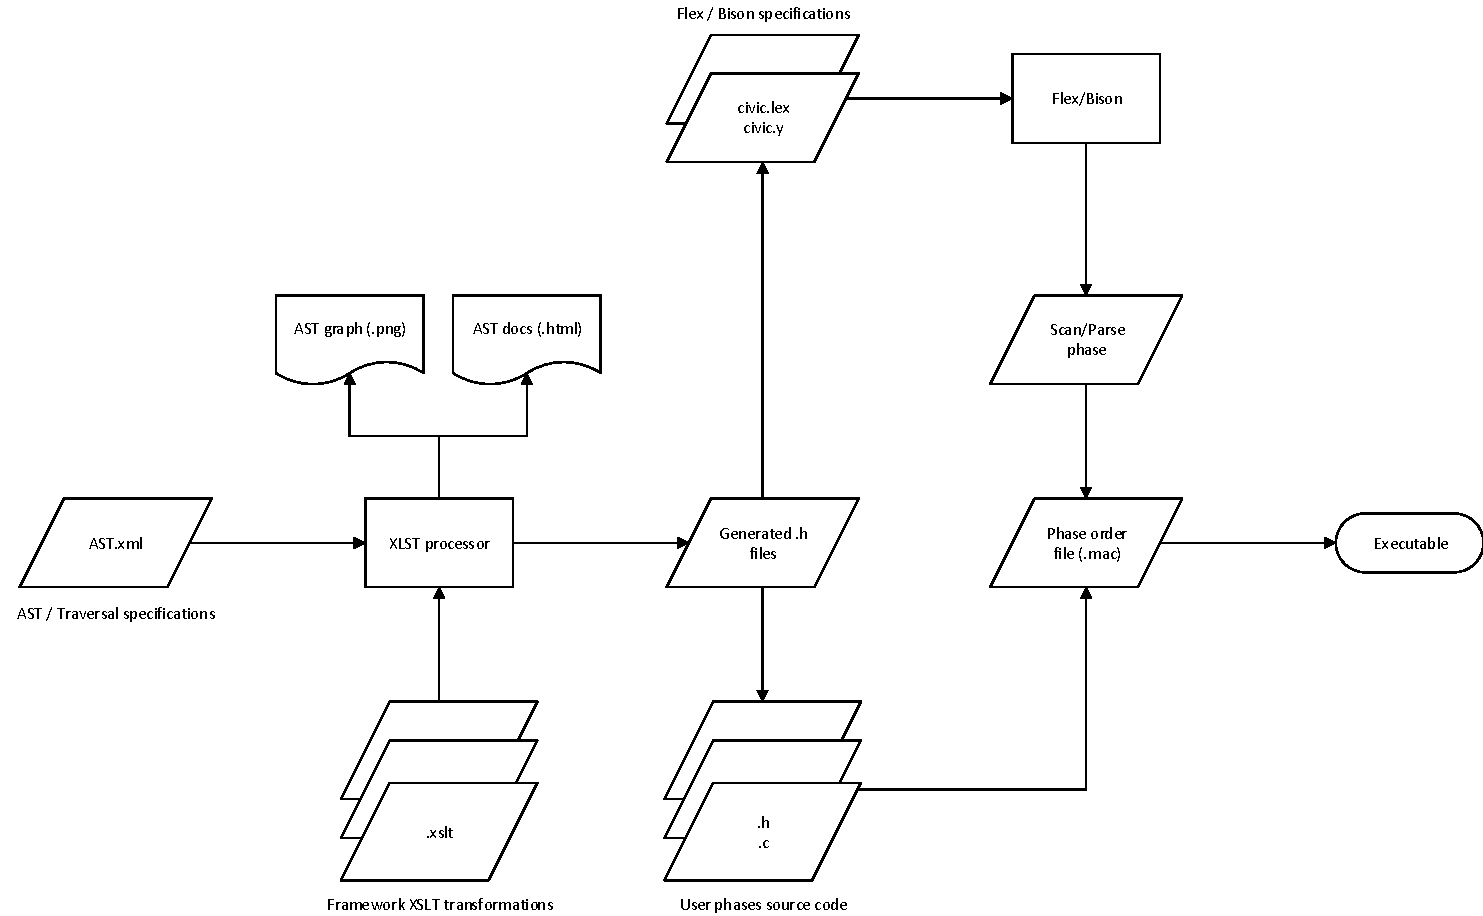
\includegraphics[width=0.95\textwidth]{figures/architecture/overview.pdf}
			\caption{Simplified overview of the Civic framework}
			\label{fig:build-dep}
		\end{figure}
		
	\section{Key Concepts}
		\subsection{Seperate Specification And Implementation}
			Central in the approach taken by the framework is the seperation of specification and implementation. Specifications are given for:
			\begin{itemize}
				\item Nodes which form the abstract syntax tree, their attributes and child nodes
				\item Mapping from friendly attribute names to C-types, and relevant methods used for copying and free-ing
				\item Node constraints on:
				\begin{itemize}
					\item Type: only certain child nodes or attribute are valid
					\item Requirement: attributes or child node must be present
				\end{itemize}
				\item Traversals, their mode of operation, affected nodes and function prefix
			\end{itemize}
			These specifications are transformed with XSLT to:
			\begin{itemize}
				\item Access macro's for nodes and their attributes
				\item Methods for initializing nodes
				\item Validity assertions
				\item User defined tree traversals and system traversals:
				\begin{itemize}
					\item Check traversal
					\item Free traversal
					\item Copy traversal
				\end{itemize}
				\item AST documentation (HTML) and graph (PNG)
			\end{itemize}
		
		\subsection{Flexible Traversals}
			How is a tree represented (internally), and how to traverse?
			
		\subsection{Tree Validation}
			How is a tree validated, and how are type errors found?
	
	\section{Development Environment}
		Error handling, pre-configured lexer+parser, debug helpers, utilitarian base library
	
	\section{Strengths \& Weaknesses}
		\label{subsec:analysis-summary}
		Weaknesses:
		\begin{itemize}
			\item C language probable cause for:
			\begin{itemize}
				\item Complicated traversal notion (due to macro's)
				\item Check traversal could be made obsolete by including type checks in macro's
				\item Free traversal (see GC)
				\item Mixing of C-related implementation details in specification
				\item Frequent use of debug helpers (doesn't help RAD)
				\item Ancient debugging, verbose code, everything global, null pointers, etc.
			\end{itemize}
			\item Platform probable cause for:
			\begin{itemize}
				\item Extensibility issues (XSLT)
				\item Architecture not obvious
				\item Large specification required for small compiler (huge XML)
				\item Documentation (due to perceived complexity)
			\end{itemize}
		\end{itemize}
		Strong points:
		\begin{itemize}
			\item Everybody knows C (but nobody knows the framework)
			\item Platform is widely supported
			\item Forces rigid structure, deviation impossible due to non-transparency
		\end{itemize}
	
	
\chapter{Design Considerations}
	Modern language, infrastructure approach, type-safety, code-based AST. Key questions:
	\begin{itemize}
		
		\item Which programming languages are realistic alternatives to the current language, keeping in mind the current experience of students?
		\item Which areas or concepts could be improved or introduced to improve the framework's efficiency?
		\begin{itemize}
			\item In what way are these concepts dependent on implementation language or on choice of architecture?
			\item Which concepts are invariant of platform or architecture?
		\end{itemize}
	\end{itemize}
	
	\section{Language}
		As established in section~\ref{subsec:analysis-summary} a large number of shortcomings can be attributed to the C programming language. 
		
		Which programming languages are realistic alternatives to the current language, keeping in mind the current experience of students?
		
		Options: Java, Scala, C\#, C++, Python, Functional (F\#, OCaml)
		
		Considerations: Student background (no functional, Java experience), New technologies accessible (ANTLR4, advanced debugging, exception handling), ease of use
		
		Choice: C\# (ANTLR, similarity to Java with more (functional) features, availability, cross-platform footnote, personal experience, managed language, extension methods)
		
		Implications for platforms: Windows, Mono, base-CLR, etc.
		
		Code based configuration of phases and AST are major differences, overall similar approach. New error handling helper methods and type-safety.
		
		Something about a modern platform.
		
		\begin{itemize}
			\item Change to a managed OOP language relieves memory allocation issues, simplifies code based AST definition
			\begin{itemize}
				\item Direct control over AST
				\item Inherent type safety
				\item More flexibility in choice of parser/lexer generator
				\item Base library removes need for wrapper methods and guarantees documentation
			\end{itemize}
			\item Code configured pipeline allows easier manipulation of phases
			\item Action based traversal formalizes and extends existing traversal process with conditionals and inheritance based actions
		\end{itemize}
	
	\section{Architecture}
		Phase based is common and works well in general (proof?), AST graph makes sense (as does docu), 
		
	\section{Code-First vs. Specification}
		Main motivator...? Disadvantages and limitations (better suited for large-scale? multiple ASTs?)
		
		The current framework fails to completely seperate specification from implementation. But even an imaginary framework which succeeds has to interface with code at some point. 
		
		Considering code and AST are directly related, improvement is to construct AST from C\# classes, offering type safety accross traversals, inheritance options and more extensibility when compared to XSLT generated code.
		
		Honorable mentions: interface based approach, attribute tagging for order of child nodes, code generation based on inheritance graph (for visitors)
		
		Language dependency: Any managed OOP language supports this construct, though C\# additionally allows easy construction of object graph using bracket notion.
		
		Platform dependency: Breaks with AST XML definition.
		
	\section{Validation}
		Type-safety is more than enough?
		
	\section{Traversals}
		Optimal way to traverse and modify a tree? Visitor pattern, algorithm seperate from structure, not much choice.
	
		Outcome: stuck with some form of visitor, more in section x..
		
	\section{Collections}
		When given a strongly typed object graph, why not utilize the built-in support of list like structures? Discussion of problems.
	
		Case with collections:
		- Node child may be node (or derived) or list of nodes
		- Discriminated union in C\# (https://stackoverflow.com/questions/3151702/discriminated-union-in-c-sharp)
		- What doesn't work: Every node is also a list of nodes
		- Cyclic dependency in inheritance (Node : IList?)
		- Advantages: easy to add, iterate and replace
		- Disadvantages: Traversal issues (can a handler return a list?), complicates everything
		
		Case without collections:
		- More natural to traversals
		- Singly-linked or doubly-linked
		- Difficult to append to or modify
		- Can be overcome with extension methods
		
		Outcome: chosen for no collection types in lists, to avoid confusion with traversals.
	
	
\chapter{Framework Changes}
	Fundamentally changed:
	\begin{itemize}
		\item Code-First vs specification (for AST, traversals and phases - also validation omitted)
		\item Managed Language
		\item Package updates
	\end{itemize}
	Untouched or adapted:
	\begin{itemize}
		\item Traversal Mechanism (added lambda)
		\item Collection representation
		\item Base lib (arguments, default ANTLR4, documentation)
	\end{itemize}
	
	\section{Code Defined AST}
		...
		
	\section{Pluggable Phases and Traversals}
		Pluggable traversals, not the actual rework. Pluggable phases, interface definition, etc.
	
	\section{Improved Traversal Mechanism}
		AST transformation through tree traversals were and still are key components of a compiler framework. The original framework relied on configuration based code generation to create the necessary traversal paths and helper methods, resulting in indirect and cumbersome configuration of traversals. 
		
		AST transformation is crucial and diverse. Operations such as type checking, code generation, variable initialization checks, etc. Could be implemented as \textit{TypeCheck()} on objects, but this doesn't scale. Type checking operations should be kept together, etc.
		
		Extrinsic visitor: Easy addition of new methods, seperation of dissimilar operators, concrete elements visited is small, trade runtime performance for reduced intrusiveness of visitor pattern (Nordman)
		
		Walkabout is exactly what I built (essense of visitor pattern).
		
		When transforming an AST, it makes sense to use a type of depth-first traversal as actions on child nodes are often dependent on the root node and less on their cousins.
		
		The visitor pattern is a well established software pattern which separates algorithm from object structure. Specifically, it tackles traversal of a structure whose objects are part of an inheritance hierarchy.
		
		In the traditional double-dispatch version this is done by adding an \textit{accept(IVisitor)} method to all participating objects which directly return control to the visitor, invoking the \textit{visit(Object)} method on the visitor determined by the run-time type (Essense of the visitor pattern).
		
		There are many variations on the visitor pattern, such as the extrinsic visitor pattern (Nordman), reflection, type test and delegate (C\# patterns), hierarchical etc (C2.com).
				
		Introduction to composite and visitor pattern, example with no inheritance.
		
		Review of existing hybrid visitor pattern, does not translate to with inheritance. Visitor may return more generic node than given. Invoked method depends on declared node type (single dispatch).
		
		Double dispatch, calling visitor method with runtime type. However:
		- does not allow handling of types higher up in the inheritance chain
		- not natively supported by C\#, even possible?
		
		Alternatives (unsure):
		- store parent in every node, but who is responsible for setting it? Lifts responsibility to handler. Which property handled?
		
		Introduce case with multiple matching methods, implies declaration order matters.
		
		Define handler:
		- type in
		- type out
		- action or function (can be method invocation)
		
		Define visitor:
		- ordered list of handlers
		- generic visitor method with reflection lookup
		
		Added features:
		- type out omitted -> wrap with return of same type
		- conditionals on handler declaration
		
		AbstractA
		/      \
		ConcreteB	ConcreteC
		|
		ConcreteB2
		
		Visitor with:
		AbstractA Visit(AbstractA node)
		ConcreteB Visit(ConcreteB node)
		AbstractA Visit(ConcreteB2 node)
		
		Goal: preserve type safety in visitor methods without using casts:
		wrong:	expr.Left = (Expression)Visit(expr.Left);
		good:	expr.Left = Visit(expr.Left);
			
		
		\subsection{Read-Only Visitor}
			...
			
		\subsection{Extrinsic Visitor}
			Suppose transformation of IntConst to Cast (both Expression) and default visit method:
			Expression Visit(IntConst node);
			T Visit(T node);
			
			Assume we have a binop node with properties Left and Right of type Expression:
			\begin{lstlisting}[caption=Spanning tree broadcast algorithm.]
var int1 = new IntConst();
var int2 = new IntConst();
var binop = new BinOp { Left = int1, Right = int2 };
			\end{lstlisting}
			
			Invoking the visitor like this results in invocation of the default Visit handler.
			\begin{lstlisting}[caption=Spanning tree broadcast algorithm.]
binop.Left = Visit(binop.Left);
			\end{lstlisting}
			
			Lets follow the Walkabout pattern for the generic visitor method:
			\begin{lstlisting}[caption=Spanning tree broadcast algorithm.]
T Visit(T node) where T : Node
{
	if (node != null)
	{
		// If this visitor has a public method for this class, with convertible return type, invoke.
		var nodeType = node.GetType();
		var method = this.GetType().GetMethod("Visit", new[] { nodeType });
		
		if (method != null \&\& (method.ReturnType == typeof(T) || method.ReturnType.IsSubclassOf(typeof(T))))
		{
			return (T) method.Invoke(this, new [] {node});
		}
		
		// Otherwise traverse children.
		VisitChildren(node);
	}
	
	return node;
}
			\end{lstlisting}
			
			Suppose default visit children method which traverses and sets child node properties:
			
			\begin{lstlisting}[caption=Spanning tree broadcast algorithm.]
void VisitChildren(Expression expr)
{
	foreach (prop of expr.GetNodeDerivativeProps())
	{
		Node value = (Node) prop.GetValue();
		if (value != null)
		{
			value = Visit(value);
			prop.SetValue(newValue);
		}
	}
}
			\end{lstlisting}
			
			GetValue() and SetValue operate on objects, the cast to Node is only required to ensure the most general case of T Visit(T node) functions.
			
			Invoking the VisitChildren method on the BinOp successfully replaces both IntConst's with Casts.
			
				Now suppose we want to write a method which acts on ALL expressions:
			Expression Visit(Expression expr);
			
			We need to establish rules on precedence. The most intuitive approach would be to assume the most concrete visitor method should be called, similar to single-dispatch.
			
			Now that we have handlers on two inheritance levels, invoking the most concrete handler involves a dynamic cast.
			\begin{lstlisting}[caption=Spanning tree broadcast algorithm.]
binop.Left = Visit((dynamic) binop.Left);
binop.Right = Visit(binop.Right);
			\end{lstlisting}
			
			VisitChildren also works because the GetMethod reflection call takes into account inheritance hierarchy.
			
			But is this approach type safe? A dynamic object is essentially something of type 'object' and exists only at compile time (MSDN). The fundamental weakness in this approach lies in the premise that a node handler can return something more abstract than itself. To introduce a run-time error all we have to do is make the IntConst handler more abstract by returning a node:
			Node Visit(IntConst node) { return new Node(); }
			
			This runtime error is thrown because the property on BinOp requires an Expression and the generic visit method has not taken this into account. The value of a property is always returned as an object, and the property field type is retrieved using reflection. This means we cannot cast to the required type resulting in a perfectly working visitor returning an object too generic.
			
			It is possible to supply this information to the Visit method without exposing it to outer classes. First the generic visitor and VisitChildren methods will be placed in an abstract class from which a new concrete visitor will inherit. Next, the visitor function is modified and made private:
			\begin{lstlisting}[caption=Spanning tree broadcast algorithm.]
T Visit(T node, Type maxUpcast) where T : Node
{
	...
	if (method != null \&\& (method.ReturnType == maxUpcast || method.ReturnType.IsSubclassOf(maxUpcast)))
	..
}
			\end{lstlisting}
			
			A wrapper method is introduced which hides this and restores the original behavior:
			\begin{lstlisting}[caption=Spanning tree broadcast algorithm.]
T Visit(T node) where T : Node
{
	return Visit(node, typeof(T));
}
			\end{lstlisting}
			
			Finally the VisitChildren function is adjusted to pass along the type of the property:
			\begin{lstlisting}[caption=Spanning tree broadcast algorithm.]
value = Visit(value, prop.PropertyType);
			\end{lstlisting}
			
			Instead of throwing a runtime error, the visitor now assumes the default case, skips invocation and jumps straight to visiting children. Static type checking is still performed by the C\# compiler, preventing this from compiling:
			\begin{lstlisting}[caption=Spanning tree broadcast algorithm.]
binop.Right = visitor.Visit((BoolConst)binop.Right);
			\end{lstlisting}
			
			The only case which is not supported in this scenario is one where there are two matching methods with differing return types:
			\begin{lstlisting}[caption=Spanning tree broadcast algorithm.]
Expression Visit(IntConst i);
IntConst Visit(IntConst i);
			\end{lstlisting}
			
			Drawbacks: always have to invoke visitor with dynamic cast when also targeting higher up the inheritance hierarchy.
			
		\subsection{Lambda Visitor}
			While this approach is sufficient for most traversals, it requires some care when multiple inheritance layers are targeted. Method invocation depends on two separate mechanisms, namely direct (single-dispatch via compiler) and reflection based. This ambiguity can be avoided by preventing direct access to visitor methods. This approach takes the decoupling from the extrinsic visitor design one step further by removing publicly defined visitor methods and replacing them with configuration functions which attach handlers.
			
			The basic traversal mechanism is the same, except instead of probing for publicly exposed methods an ordered list of handlers is consulted instead. This also prevents ambiguity when multiple layers of inheritance are targeted by explicitly stating the order of evaluation. Such handlers must contain at least:
			\begin{enumerate}
				\item Type of the node handled
				\item Return type of the handler (similar to the upcast restraint)
				\item Delegate containing the transformation function
			\end{enumerate}
			
			The previous distinction between methods which replace nodes and those who only act on them can be removed by offering two types of delegates. In .NET these are represented by the Func<T, T> and Action<T>  delegates, indicating respectively a function which takes an object of type T and returns an object of type T and a function which takes an object of type T but doesn't return anything. These can be interleaved as in returning nothing in essence indicates no change to the initial object; it would behave 'as-if' it would return itself.
			
			Considering the logic determining which visitor function should be invoked is now entirely encapsulated by the visitor itself, a simple but useful feature would be an optional predicate preceding invocation of the function. This, together with a lambda-style approach to defining visitor methods allows for more configuration flexibility. Such handlers must additionally hold:
			\begin{enumerate}
				\setcounter{enumi}{3}
				\item Return type of the delegate
				\item Delegate containing a predicate
			\end{enumerate}
			
			\includecode{Test}{report.bib}
			
			Additionally, fall-through handlers could be supported with this approach. The decision not to do so is based on the fact that fall-through statements have been mostly banned from the switch construct in modern imperative languages such as Java and C\#. The recent HeartBleed-bug in OpenSSL was also caused by an improperly handled fall-through.
			
			Suppose we have two handlers (in-order):
			F(IntConst, Node)
			F(IntConst, Expression)
			
			In the BinOp example previously defined the second handler would be invoked as they are held in properties of type Expression. 
			
			Adding 
			
	\section{Development Environment}
		Implications of unmanaged vs managed, reduction of base library, debug upgrade..?
		
		\subsection{Updated Lexer/Parser}
			More flexible Parser/Lexer generator support, such as ANTLR4 (LL(*) with EBNF).
			
			Language dependency: Plenty of parsers exist for any language, first version of AST most likely constructed in code; change of language not essential.
			
			Platform dependency: Depends on extensibility of parser generator, ANTLR4 has multiple ways of traversing a generated parse tree, YACC does not (embedding of code in parse phase restricts construction of AST)
			
		\subsection{Platform Updates}
			NuGet
			
		\subsection{Documentation Generator}
			Inheritance graph plotter, AST graph plotter
	
	
\chapter{Discussion}
	Key questions:
	\begin{itemize}
		\item Which aspects of the existing framework are a result of language?
		\item How does the new framework differ from other compiler platforms?
		\item What other factors could improve the efficiency of the framework?
	\end{itemize}
	
	- vNext immutable AST
	- 

\bibliography{report}
\bibliographystyle{plainnat}
\end{document}